\cia \vspace{-2cm}
\section{Missing mass cuts}

Background coming from a residual $ep\rightarrow e'p'\gamma $
and from two pion production processes has been taken into account
in the calculation of the systematic errors by varying the missing mass cut according
to Table \ref{tab:missing_mass_cuts}.


\begin{table}[h]
 \begin{center}
  \begin{tabular}{c | c}
    & \\
    min ($GeV^2$)  &  max ($GeV^2$)  \\ 
    & \\
    \hline
    & \\
    -0.05  & 0.08  \\
    -0.04  & 0.075 \\ 
    -0.04  & 0.07  \\
    -0.03  & 0.065 \\
    -0.02  & 0.06  \\
    & \\
    \hline
  \end{tabular}
 \end{center} 
 \caption{ Missing mass cuts}
 \label{tab:missing_mass_cuts}
\end{table}

The cuts are illustrated in \F{fig:mmcuts}.

\begin{figure}[h]
 \begin{center}
  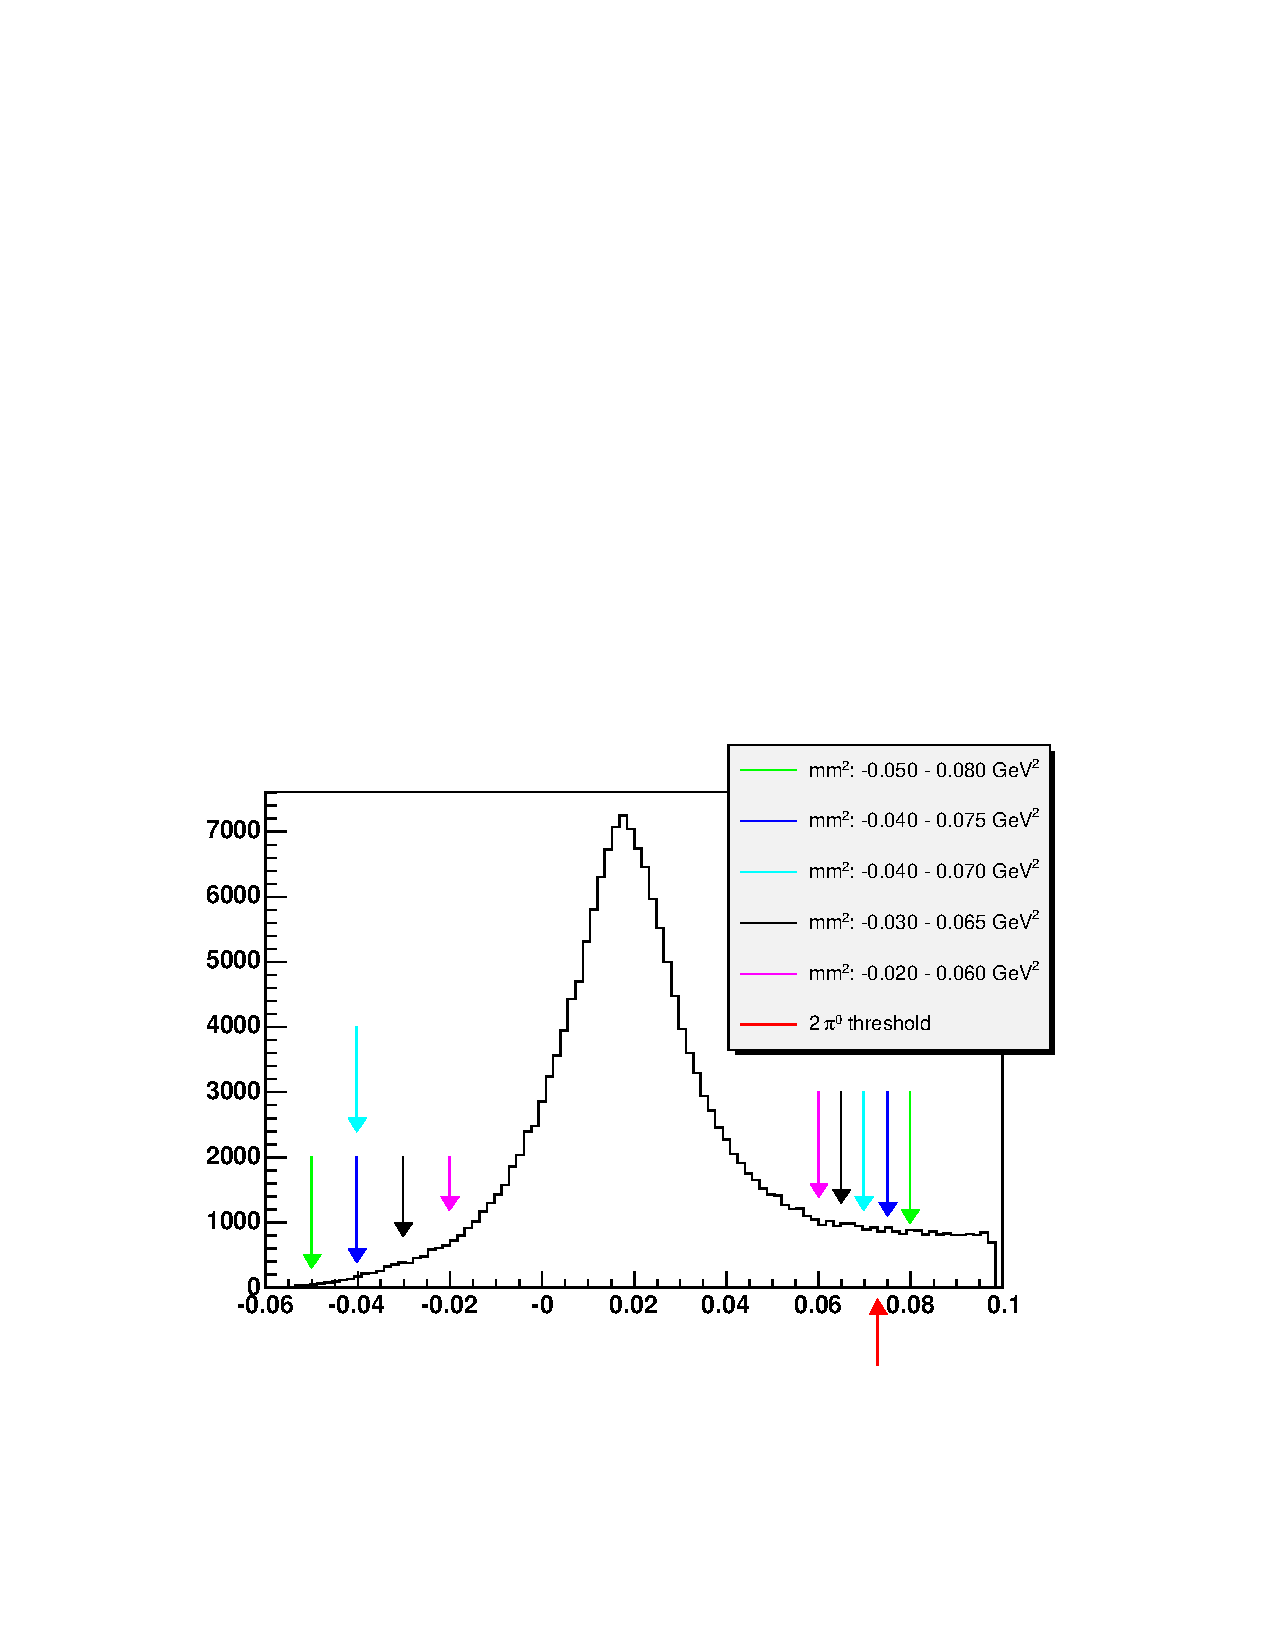
\includegraphics[width = 11cm, bb = 80 140 540 480]{systematics/img/mmcuts}
  \caption{ Missing mass square distribution for $\pi^0$ events and the different
            cuts used for the systematic study. }
  \label{fig:mmcuts}
 \end{center}
\end{figure} 

The variation of the ratios $R_{EM}$ and $R_{SM}$ for the first and last cut is illustrated in 
\F{fig:ratios_mm_syst}.
\begin{figure}[h]
 \begin{center}
  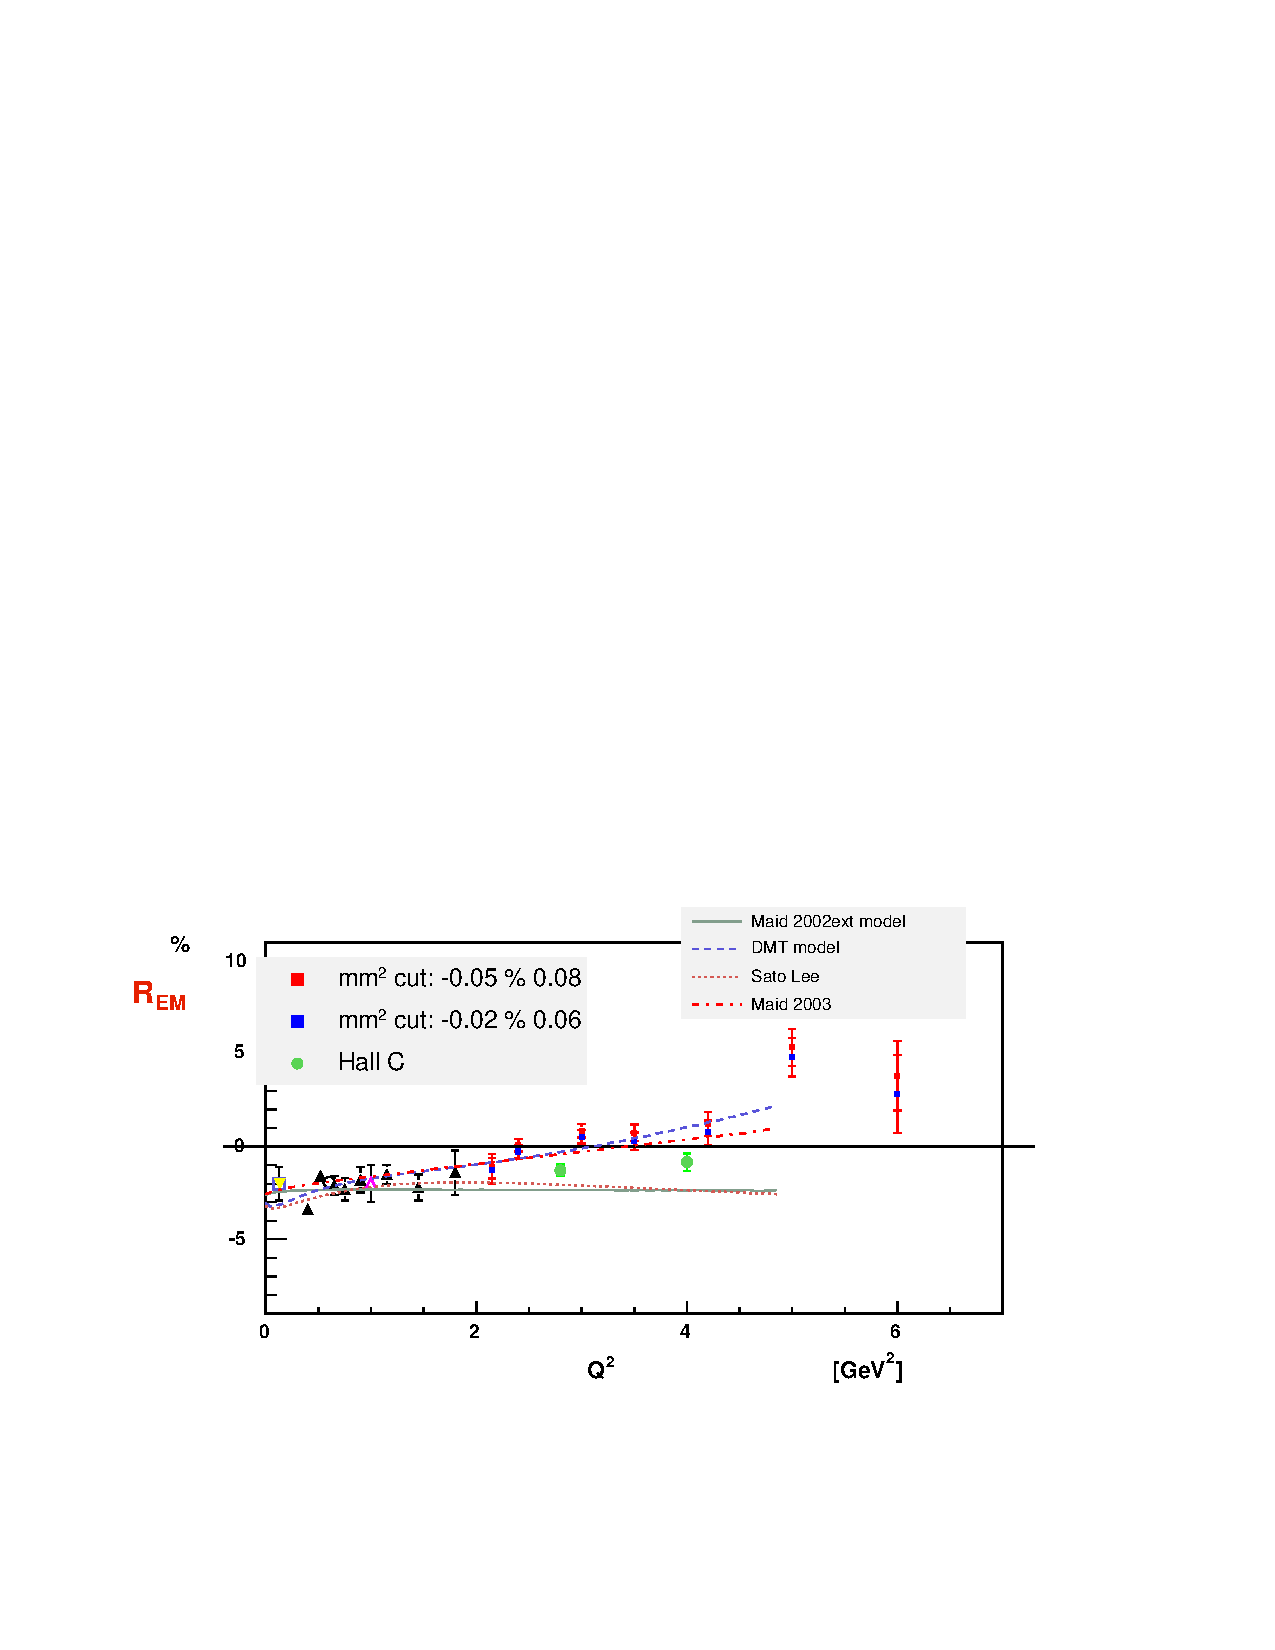
\includegraphics[width = 12cm, bb = 50 120 540 440]{systematics/img/rem_mmsyst}
  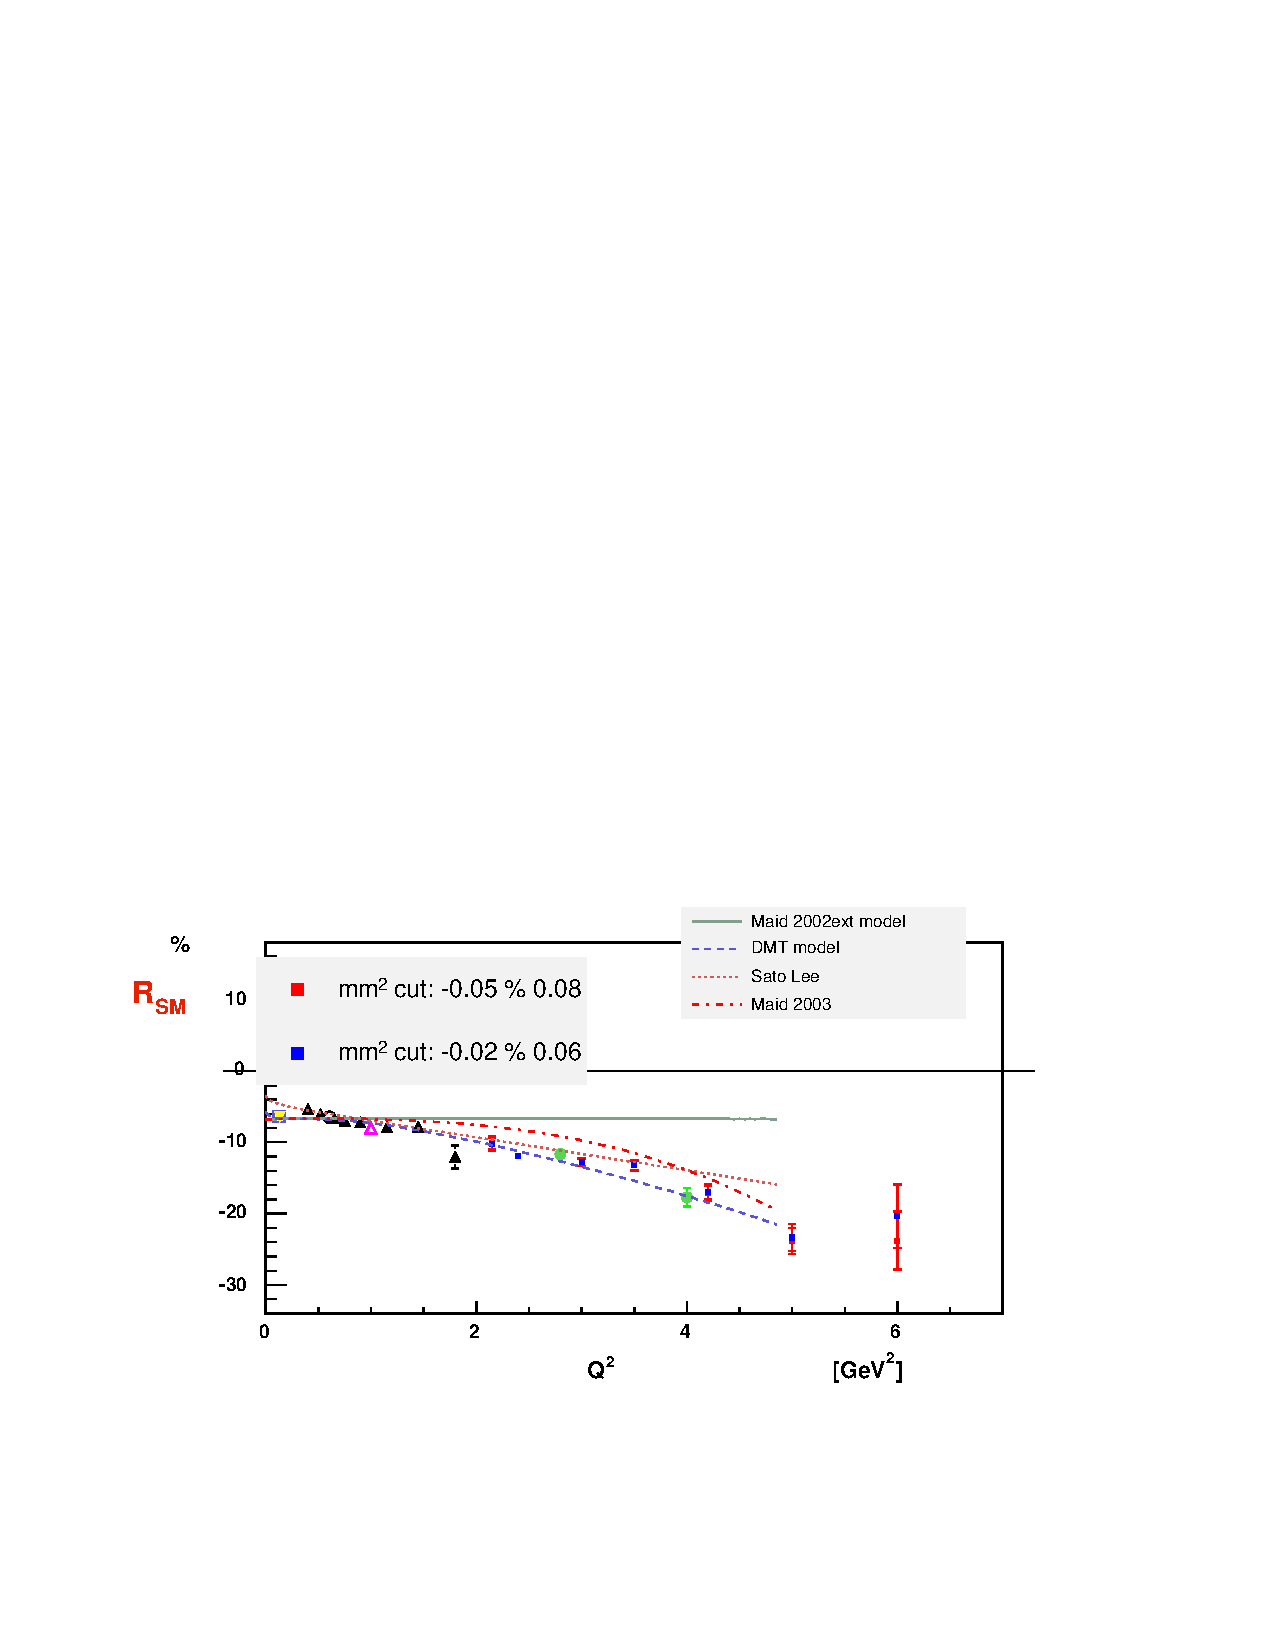
\includegraphics[width = 12cm, bb = 50 100 540 440]{systematics/img/rsm_mmsyst}
  \caption{ Variation of the ratios $R_{EM}$ (top) and $R_{SM}$ (bottom) for the missing mass square cuts:
           $-0.05 < mm^2 < 0.08$ and $-0.02 < mm^2 < 0.06$ }
  \label{fig:ratios_mm_syst}
 \end{center}
\end{figure} 






